\documentclass{article}
\usepackage{iclr2027_conference,times}

\input{math_commands.tex}
% Shared notation. Edit here rather than repeating in the body.
\newcommand{\znow}{z_{\mathrm{now}}}
\newcommand{\zg}{z_{g}}
\newcommand{\planlen}{25}
\newcommand{\Fk}{F^{k}}
\newcommand{\Bk}{B^{k}}


\usepackage{hyperref}
\usepackage{url}
\usepackage{graphicx}
\usepackage{booktabs}
\usepackage{amssymb}

\title{FBLeWM: Forward and Backward Latent Imaginers\\
for Short-Horizon CEM Planning}

% Hidden on submission (double-blind). Uncomment \iclrfinalcopy for camera-ready.
\author{Anonymous authors \\
Paper under double-blind review}

\newcommand{\fix}{\marginpar{FIX}}
\newcommand{\new}{\marginpar{NEW}}

% \iclrfinalcopy % Uncomment for camera-ready, NOT for submission.

\begin{document}

\maketitle

\begin{abstract}
% One paragraph. Locked claim: F/B give a 25-step CEM a longer-range ranking
% signal; we do not claim calibrated $F^{k}(p)\approx z_{t+k}$.
\end{abstract}

\section{Introduction}
\label{sec:intro}

\section{Related work}
\label{sec:related}

LeWM~\citep{lewm2026} trains an encoder $E$, an action-conditioned predictor $P$, and a CEM planner with next-embedding MSE plus SIGReg. FBLeWM keeps this official path unchanged and adds two detached action-free imaginers.

\section{Method}
\label{sec:method}

\subsection{Official LeWM (unchanged)}
\[
\mathcal{L}_{\mathrm{official}}
=\underbrace{\|P(z,a)-z_{\mathrm{next}}\|^2}_{\mathrm{pred}}
+0.09\,\mathcal{L}_{\mathrm{SIGReg}}(z).
\]
CEM always plans $\planlen$ environment steps.

\subsection{Detached imaginers}
Forward and Backward read stop-gradient latents. Their losses do not update $E$ or $P$.

\paragraph{Forward.}
$F(p)\to z$ (unary). At evaluation,
\[
C_{F}=\bigl\|\Fk\bigl(P_{25}\bigr)-\zg\bigr\|^2.
\]

\paragraph{Backward (unary, $B\to z$; figures in this draft).}
$B(z_{t+1})\to z_t$. At evaluation,
\[
C_{B}=\bigl\|P_{25}-\Bk(\zg)\bigr\|^2.
\]

\paragraph{Backward (conditional, \texttt{now}; TwoRoom v2, not in figures yet).}
\[
g\leftarrow B(z_0,g),\qquad
B(z_0,z_3)\to z_2,\quad
B(z_0,z_2)\to z_1.
\]

\paragraph{Imagination depth.}
\[
k=\max\bigl((o-t-\planlen)/5,\,0\bigr)
\quad\text{(goal offset $o$, elapsed $t$, action block $5$).}
\]
When $k=0$, $F$ and $B$ are bypassed and the cost matches Official.

\paragraph{Fusion (avg05).}
$C=0.5\,C_F+0.5\,C_B$.

\section{Experiments}
\label{sec:exp}

Protocol: $n{=}50$, seed $42$, shared starts within each task, checkpoint at epoch 10, CEM horizon $5$ unless noted. Success is the environment criterion, not latent MSE.

% Number lookup while writing: ../outputs/figures/FIGURES.md

\subsection{PushT}
\label{sec:pusht}

\begin{table}[t]
\caption{PushT success (\%). CEM${=}5$ at all offsets. Same 50 starts.
Checkpoint \texttt{fblewm} (unary $B\to z$).}
\label{tab:pusht}
\begin{center}
\begin{tabular}{lcccc}
\toprule
Mode & 25 & 50 & 75 & 100 \\
\midrule
Official        & 82 & 44 & 22 & 12 \\
Forward         & 82 & 62 & 42 & 28 \\
Backward        & 82 & 70 & 34 & 10 \\
Fusion (avg05)  & 82 & 78 & 50 & 18 \\
\bottomrule
\end{tabular}
\end{center}
\end{table}

\begin{figure}[t]
\begin{center}
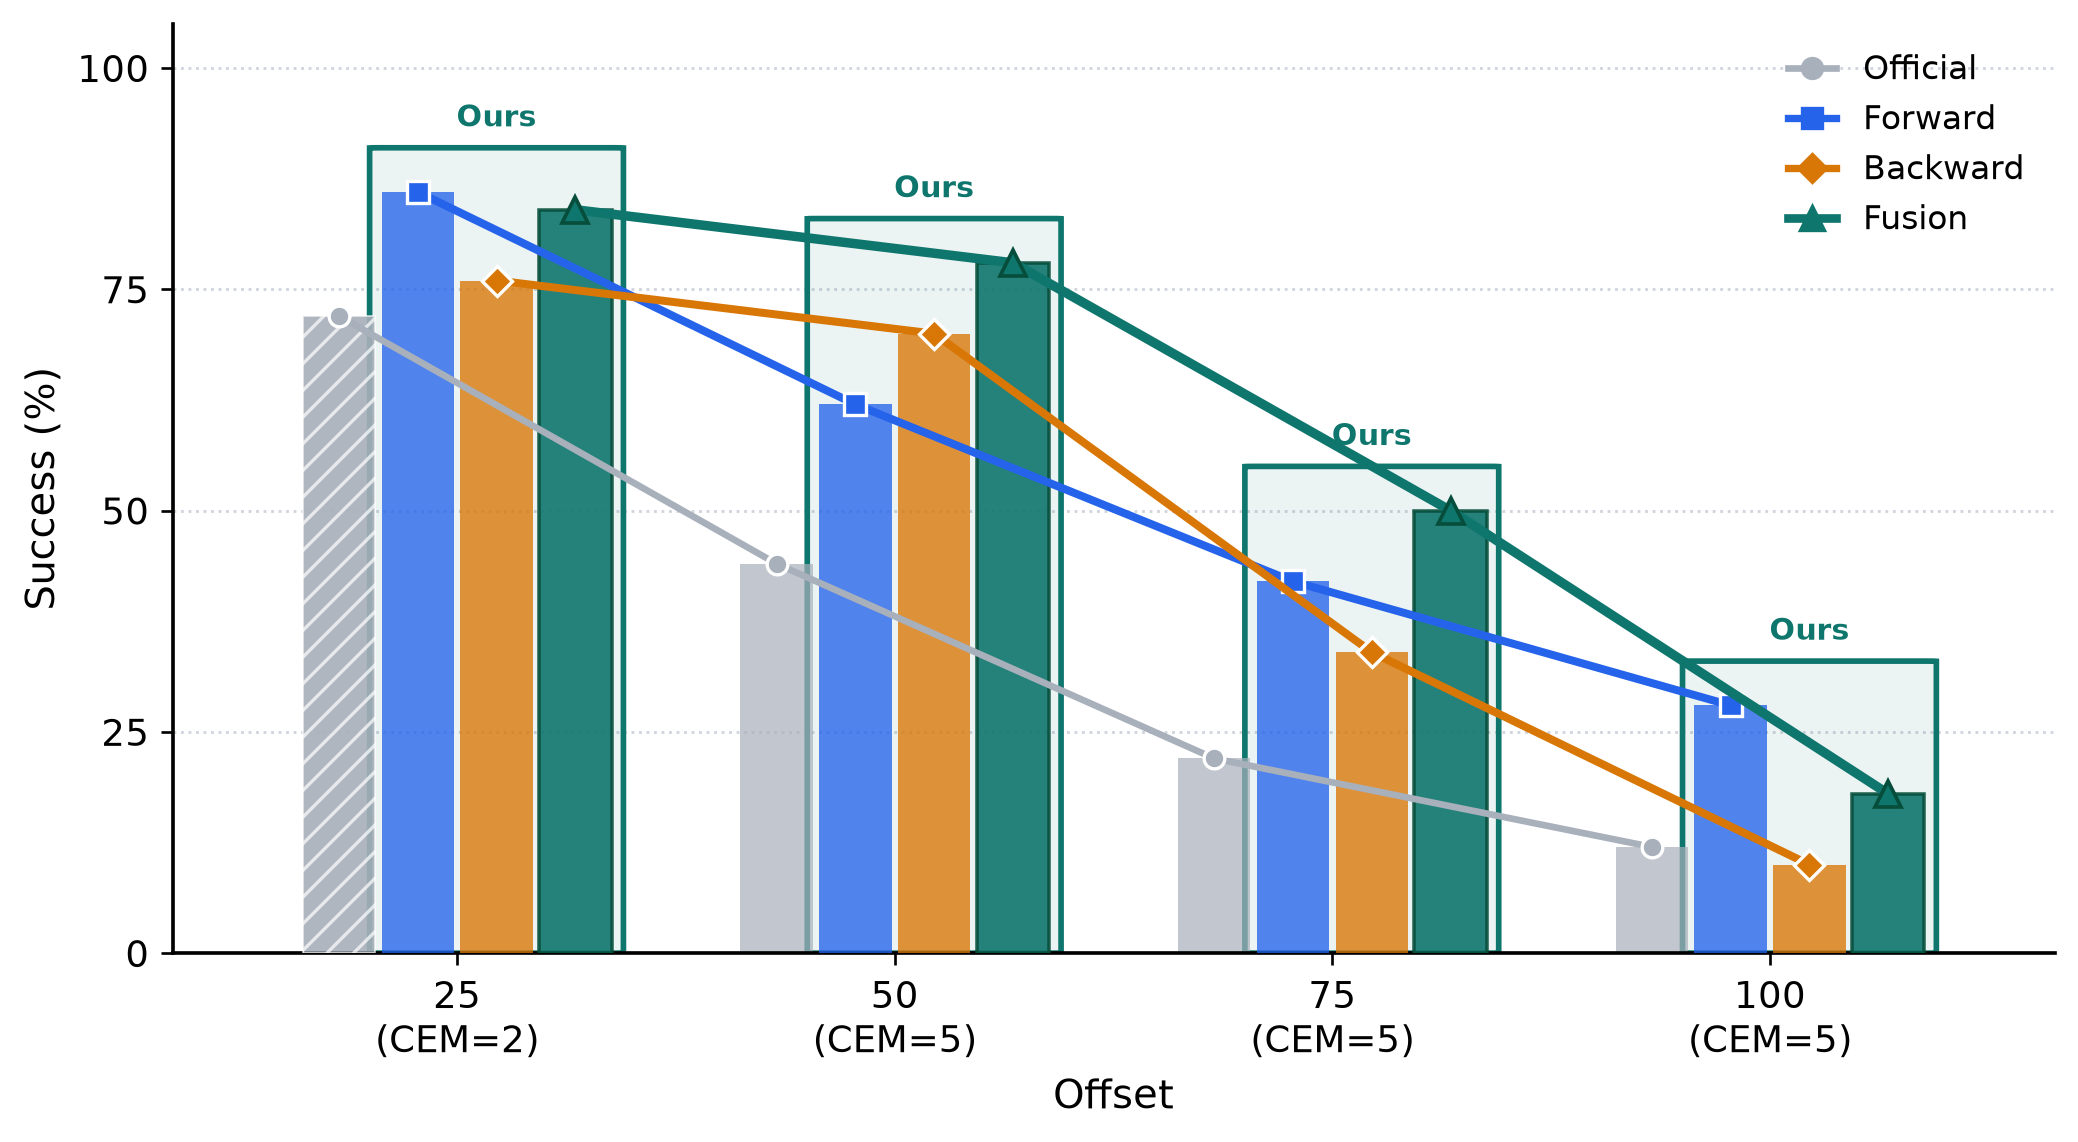
\includegraphics[width=\linewidth]{figures/fig_pusht_success.png}
\end{center}
\caption{PushT success vs.\ offset. This PNG uses CEM horizon $2$ at offset $25$ (Official $72$, Forward $86$); offsets $50$--$100$ match Table~\ref{tab:pusht}. If the paper protocol is CEM${=}5$ everywhere, quote the table at offset $25$ ($82/82/82/82$), not the bars.}
\label{fig:pusht-success}
\end{figure}

\begin{figure}[t]
\begin{center}
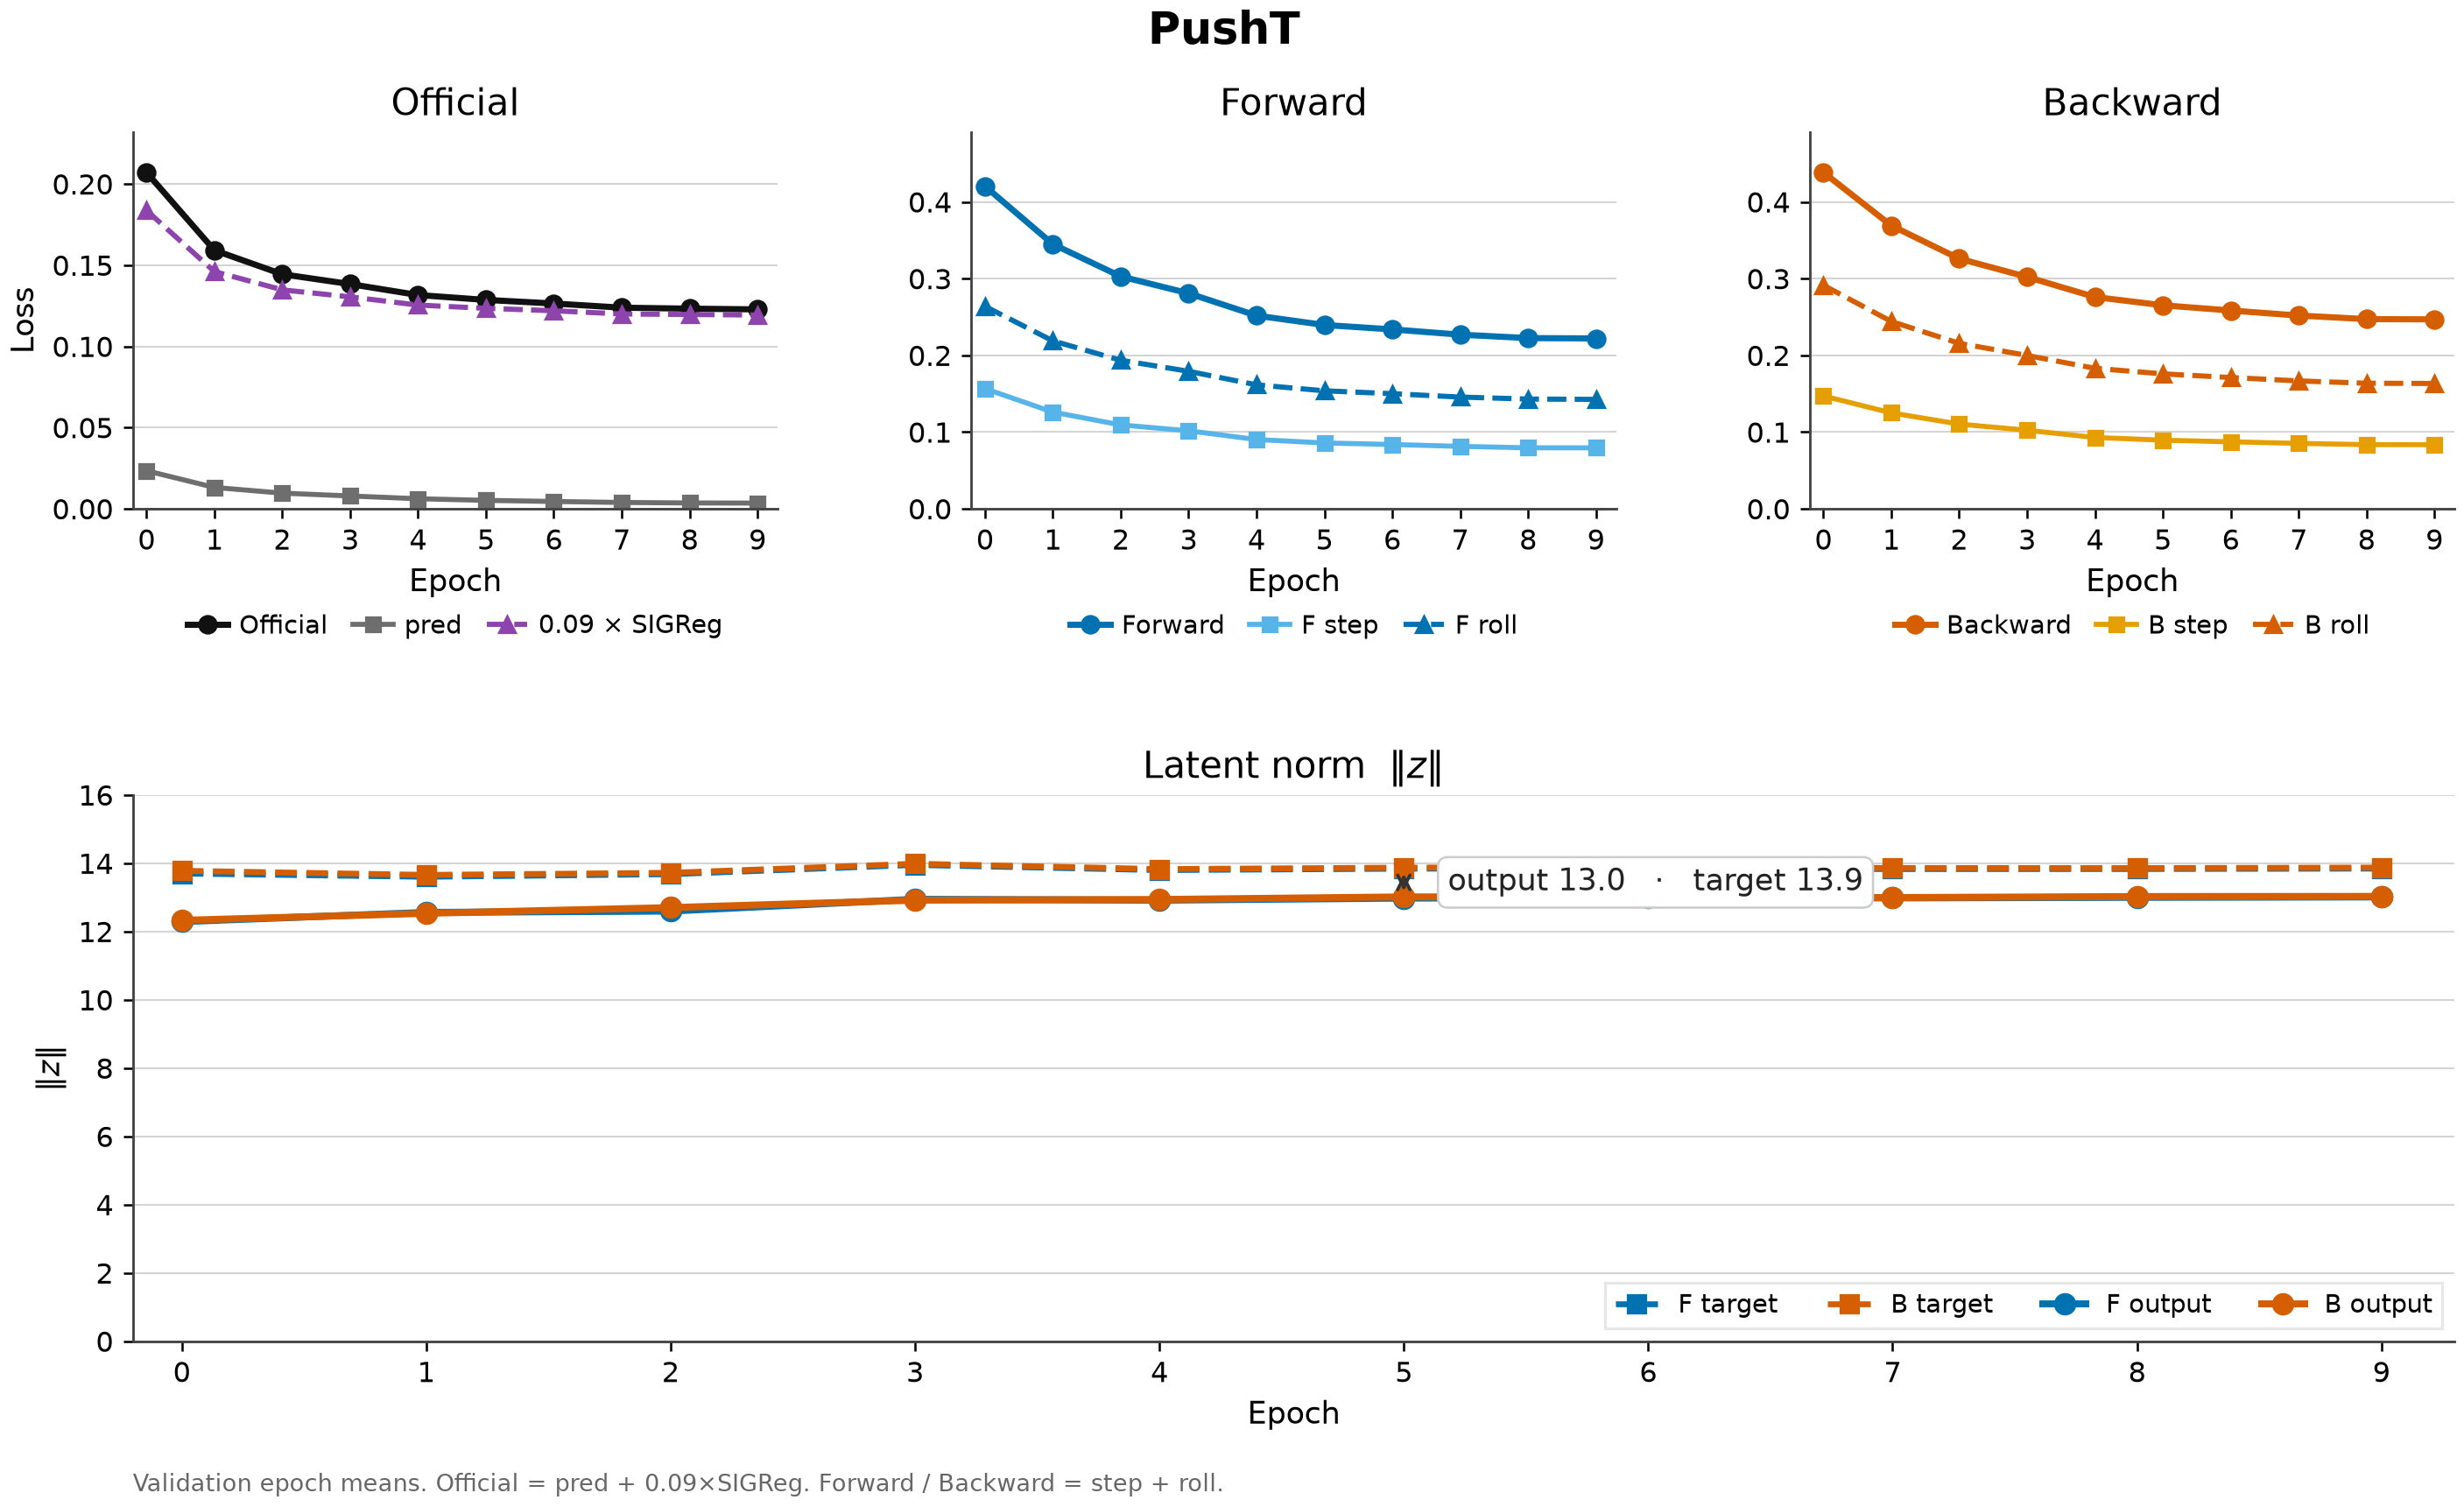
\includegraphics[width=\linewidth]{figures/fig_pusht_train.png}
\end{center}
\caption{PushT validation losses and latent norms. F/B outputs stay near the BatchNorm sphere ($\Vert z\Vert{\approx}\sqrt{192}{\approx}13.9$).}
\label{fig:pusht-train}
\end{figure}

\subsection{TwoRoom}
\label{sec:tworoom}

\begin{table}[t]
\caption{TwoRoom success (\%). CEM${=}5$ at all offsets. Same 50 starts.
Checkpoint \texttt{fblewm\_tworoom} (unary $B\to z$).}
\label{tab:tworoom}
\begin{center}
\begin{tabular}{lcccc}
\toprule
Mode & 25 & 50 & 75 & 100 \\
\midrule
Official        & 90 & 50 & 32 & 18 \\
Forward         & 90 & 90 & 84 & 66 \\
Backward        & 92 & 54 & 40 & 24 \\
Fusion (avg05)  & 90 & 76 & 58 & 32 \\
\bottomrule
\end{tabular}
\end{center}
\end{table}

\begin{figure}[t]
\begin{center}
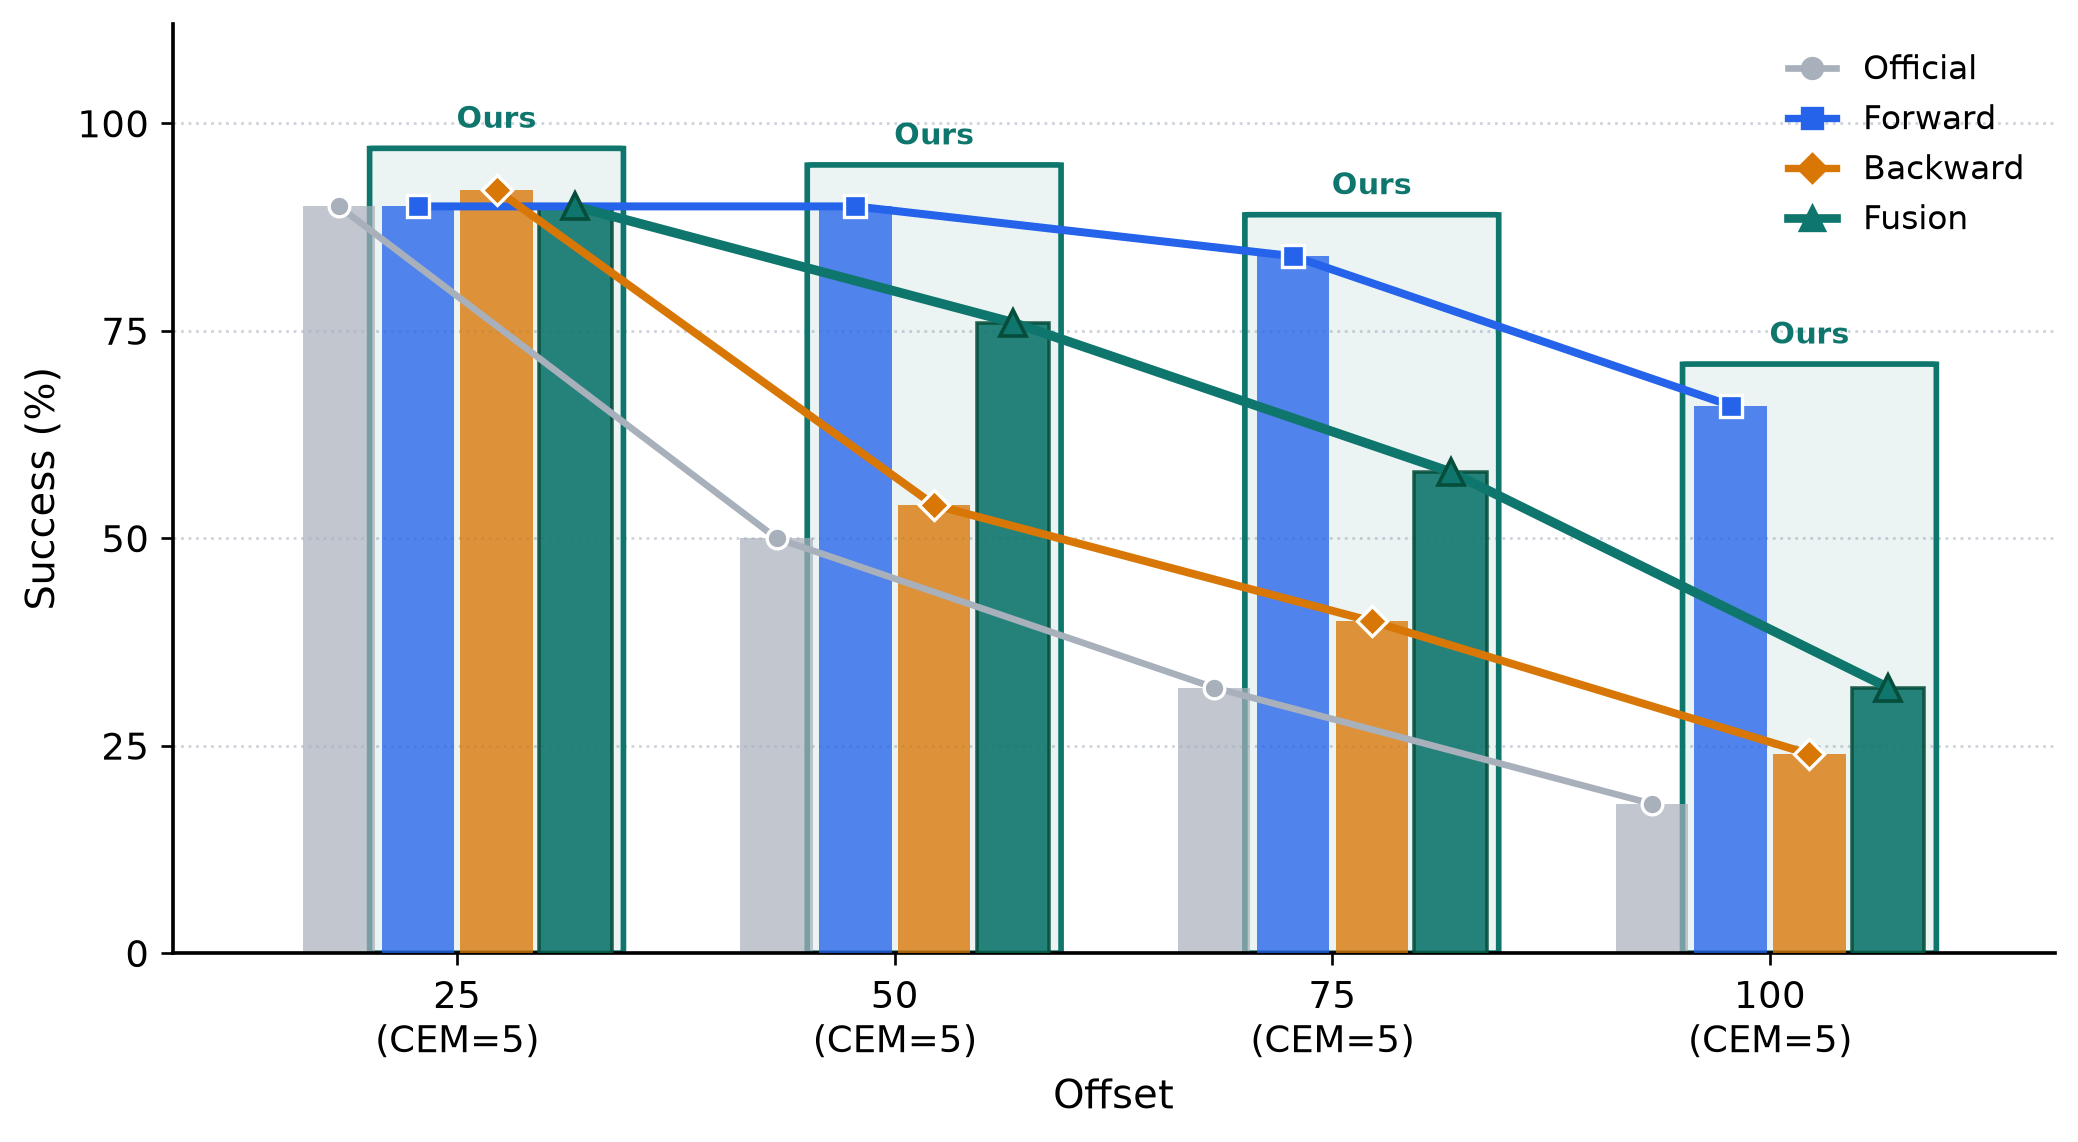
\includegraphics[width=\linewidth]{figures/fig_tworoom_success.png}
\end{center}
\caption{TwoRoom success vs.\ offset (CEM${=}5$). Forward recovers long-offset success; Fusion does not beat Forward.}
\label{fig:tworoom-success}
\end{figure}

\begin{figure}[t]
\begin{center}
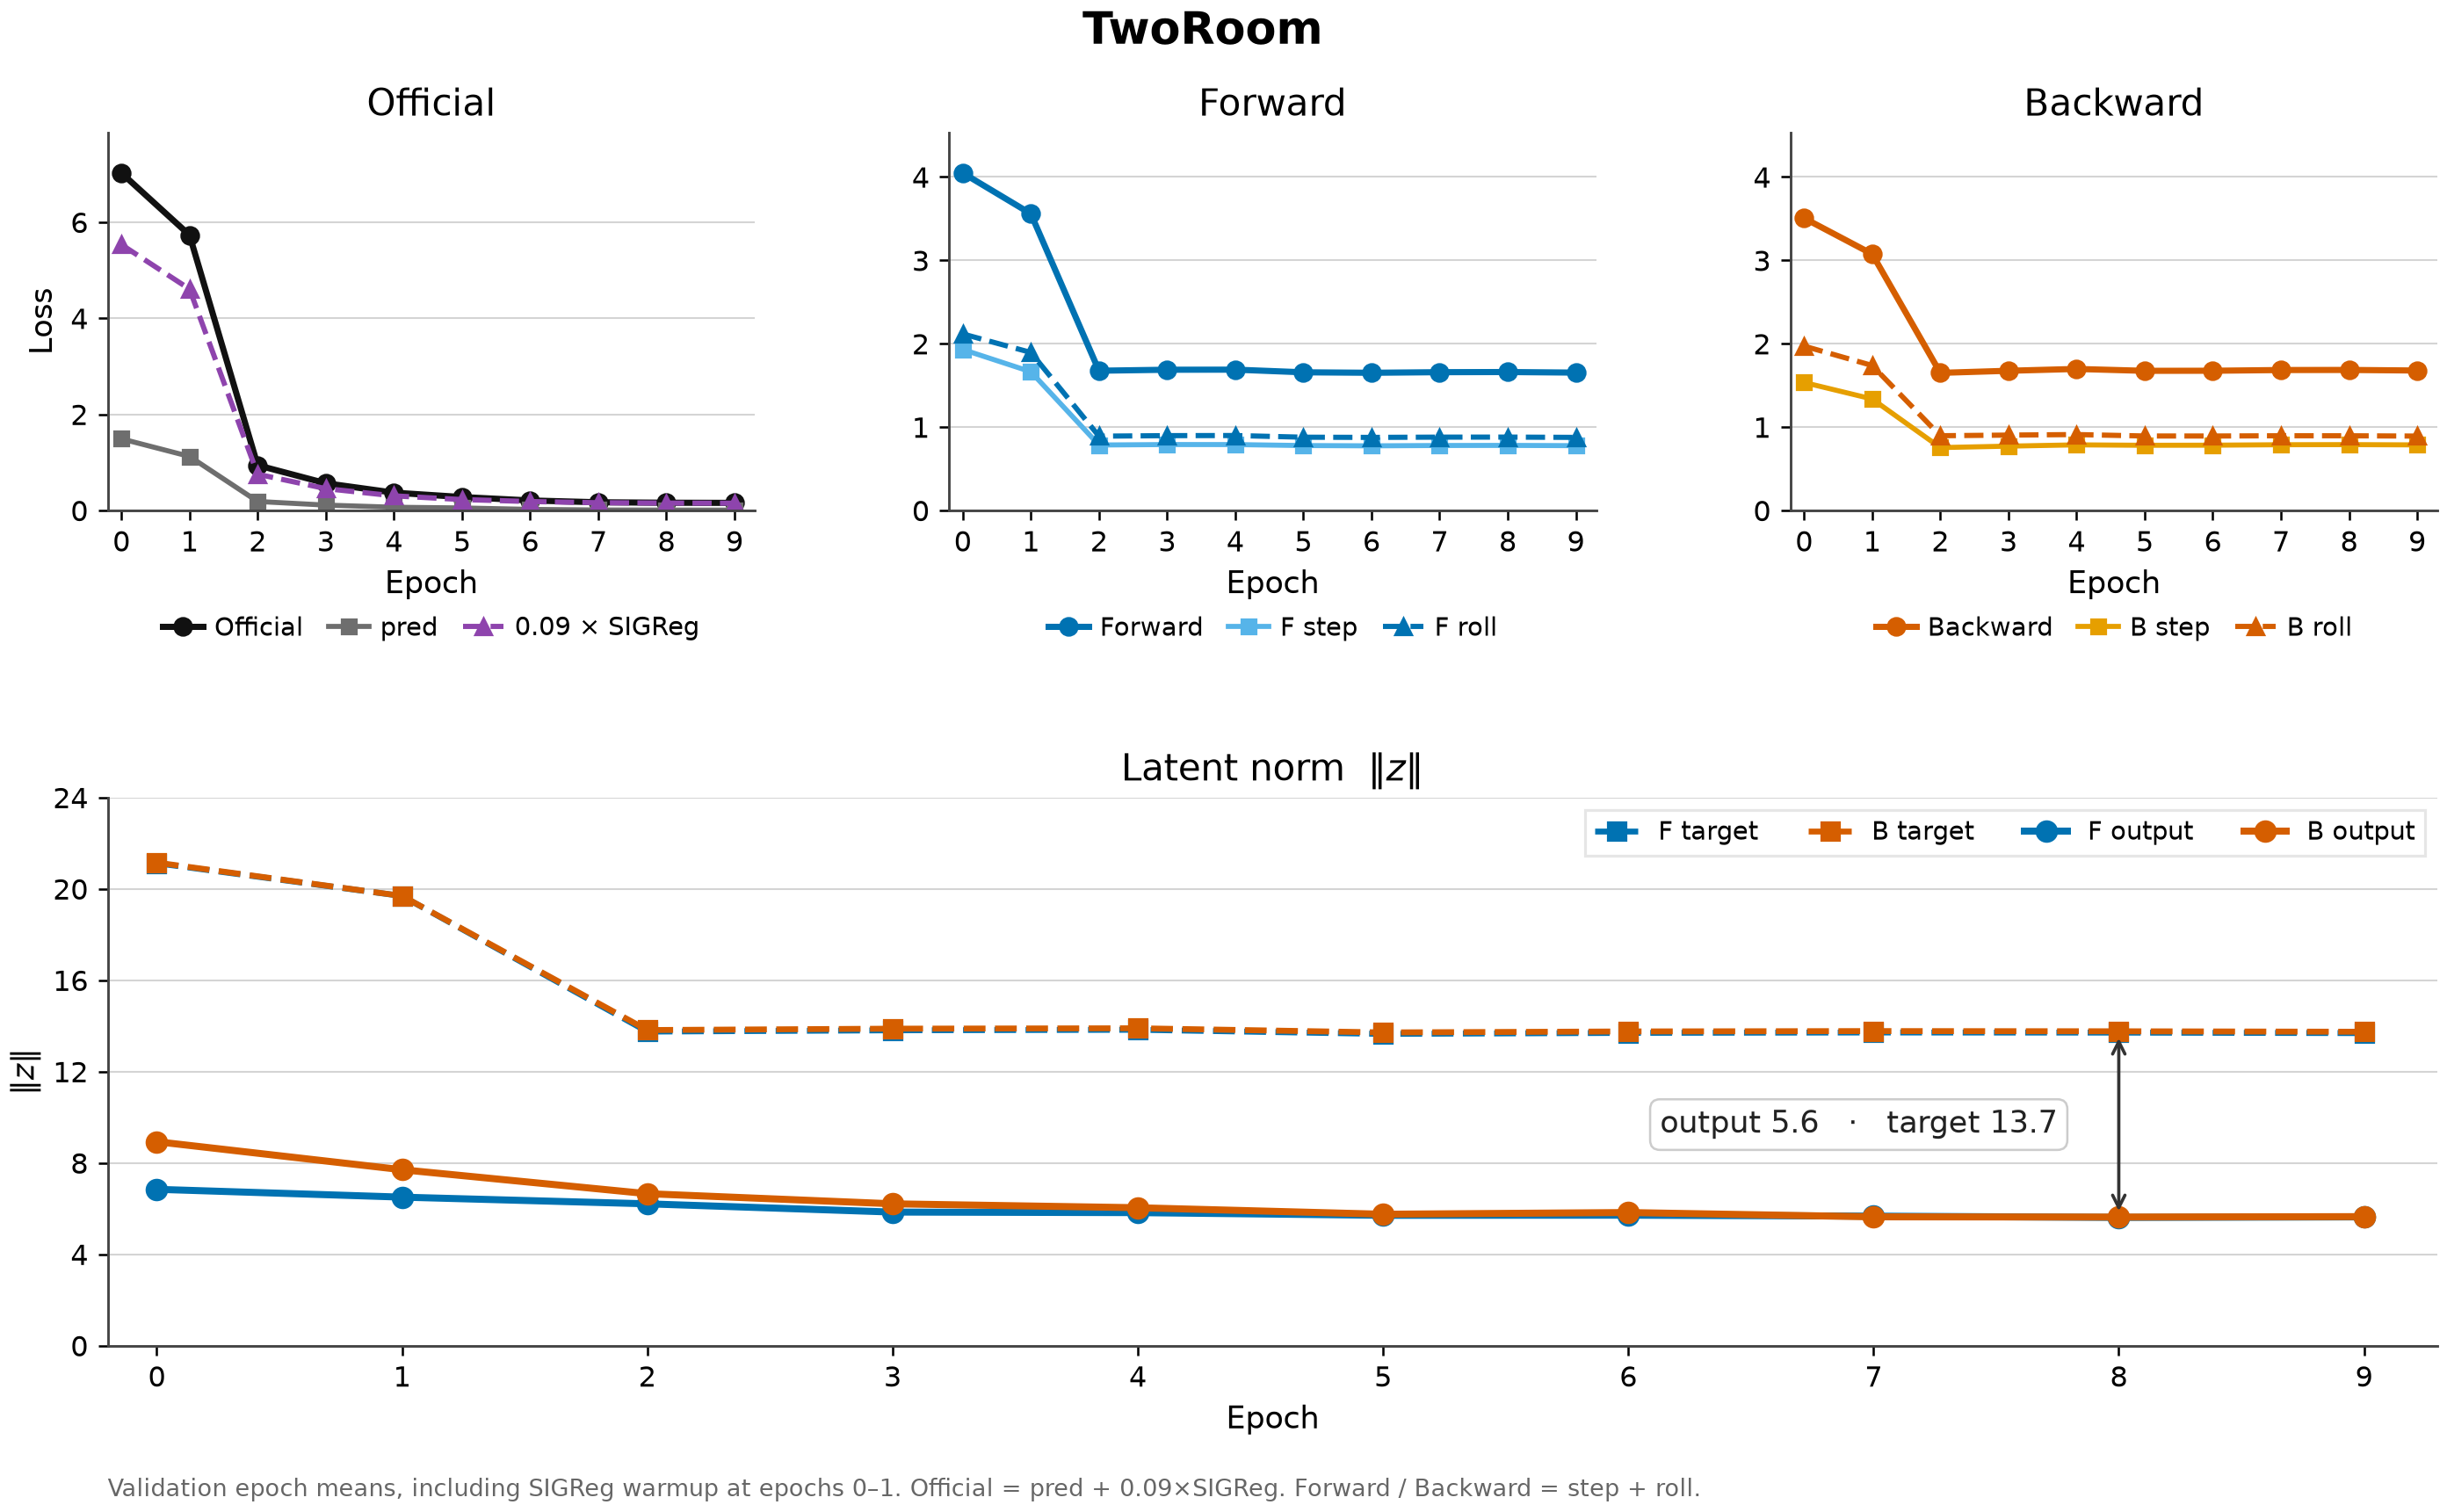
\includegraphics[width=\linewidth]{figures/fig_tworoom_train.png}
\end{center}
\caption{TwoRoom validation losses and latent norms, including SIGReg warmup at epochs $0$--$1$. After the encoder settles, F/B outputs remain ${\approx}5.6$ vs.\ target ${\approx}13.7$. Planning success in Table~\ref{tab:tworoom} still holds: ranking can survive a scale gap.}
\label{fig:tworoom-train}
\end{figure}

\subsection{Cube}
\label{sec:cube}

% Dataset archive SHA-checked. Not extracted / trained yet.

\section{Conclusion}
\label{sec:concl}

\subsection*{AI use statement}

(This section is required and does not count toward the page limit. Edit before submission; see the ICLR 2027 AI Policy for Authors.)

We used generative AI tools for code assistance and for checking grammar. We take responsibility for the final content of this work, including text, claims, and artifacts.

\subsection*{Reproducibility statement}

(This section is recommended and does not count toward the page limit.)

Training and evaluation protocols, shared starts, and numeric tables are specified in Section~\ref{sec:exp}. Source code and configs will be included as anonymous supplementary material.

\bibliography{refs}
\bibliographystyle{iclr2027_conference}

\appendix
\section{Additional results}
\label{app:extra}

% Extra fusion modes, B$\to$p ablation, CEM-horizon ablation.

\end{document}
